\chapter{पेशियाँ और संधियाँ}\label{ch:g10:muscles-and-joints}

कोई फ़ुटबॉल खिलाड़ी पैर जमाता है, मुड़ता है, और घुटना पकड़कर गिर पड़ता है।
घंटे भर बाद निदान: फटा हुआ \omterm{def:g10:muscles-and-joints:joint}{स्नायु}। हड्डियों में कुछ नहीं टूटा, कोई पेशी
नहीं चूकी; कुछ सेंटीमीटर लंबी ऊतक की एक पट्टी, जिसका काम दो हड्डियों को
एक सीध में थामे रखना था, ऐसे मरोड़ के नीचे बैठ गई जिसके लिए वह कभी बनी ही
नहीं थी। क्या फटा और घुटने को ठीक होने में महीने क्यों लगेंगे, यह समझने
के लिए हमें जानना होगा कि \omterm{def:g10:muscles-and-joints:joint}{संधि} बनी किस चीज़ से है, पेशियाँ उस पर खींच कैसे
लगाती हैं, और सत्तर किलोग्राम का शरीर एक टाँग पर उतरे तो उसमें से कौन-से
बल गुज़रते हैं।

\section{संधि}

\begin{definition}[संधि]\label{def:g10:muscles-and-joints:joint}
\emph{संधि}\index{संधि} वह जगह है जहाँ दो हड्डियाँ मिलती हैं। घुटने,
कूल्हे, कंधे या कोहनी जैसी चलायमान संधि में हड्डियों के सिरे कुछ
मिलीमीटर मोटी चिकनी \emph{उपास्थि}\index{उपास्थि} की परत से ढँके रहते
हैं, और एक बंद थैली, यानी \emph{संपुट}, में घिरे होते हैं, जिसकी भीतरी
परत वह \emph{श्लेष द्रव} स्रावित करती है जो सतहों को चिकना रखता है।
सख़्त ऊतक की पट्टियाँ, यानी \emph{स्नायु}\index{स्नायु}, संधि को लाँघकर
एक हड्डी से दूसरी तक जाती हैं और उसकी हलचल को मंशा भर तक सीमित रखती हैं।
घुटने में उपास्थि के दो अर्धचंद्रक, यानी \emph{अर्धचंद्रक}, हड्डियों के
बीच बैठते हैं और भार फैला देते हैं।
\end{definition}

\begin{omfigure}
\begin{tikzpicture}
  \node[anchor=south west, inner sep=0] (img) at (0,0)
    {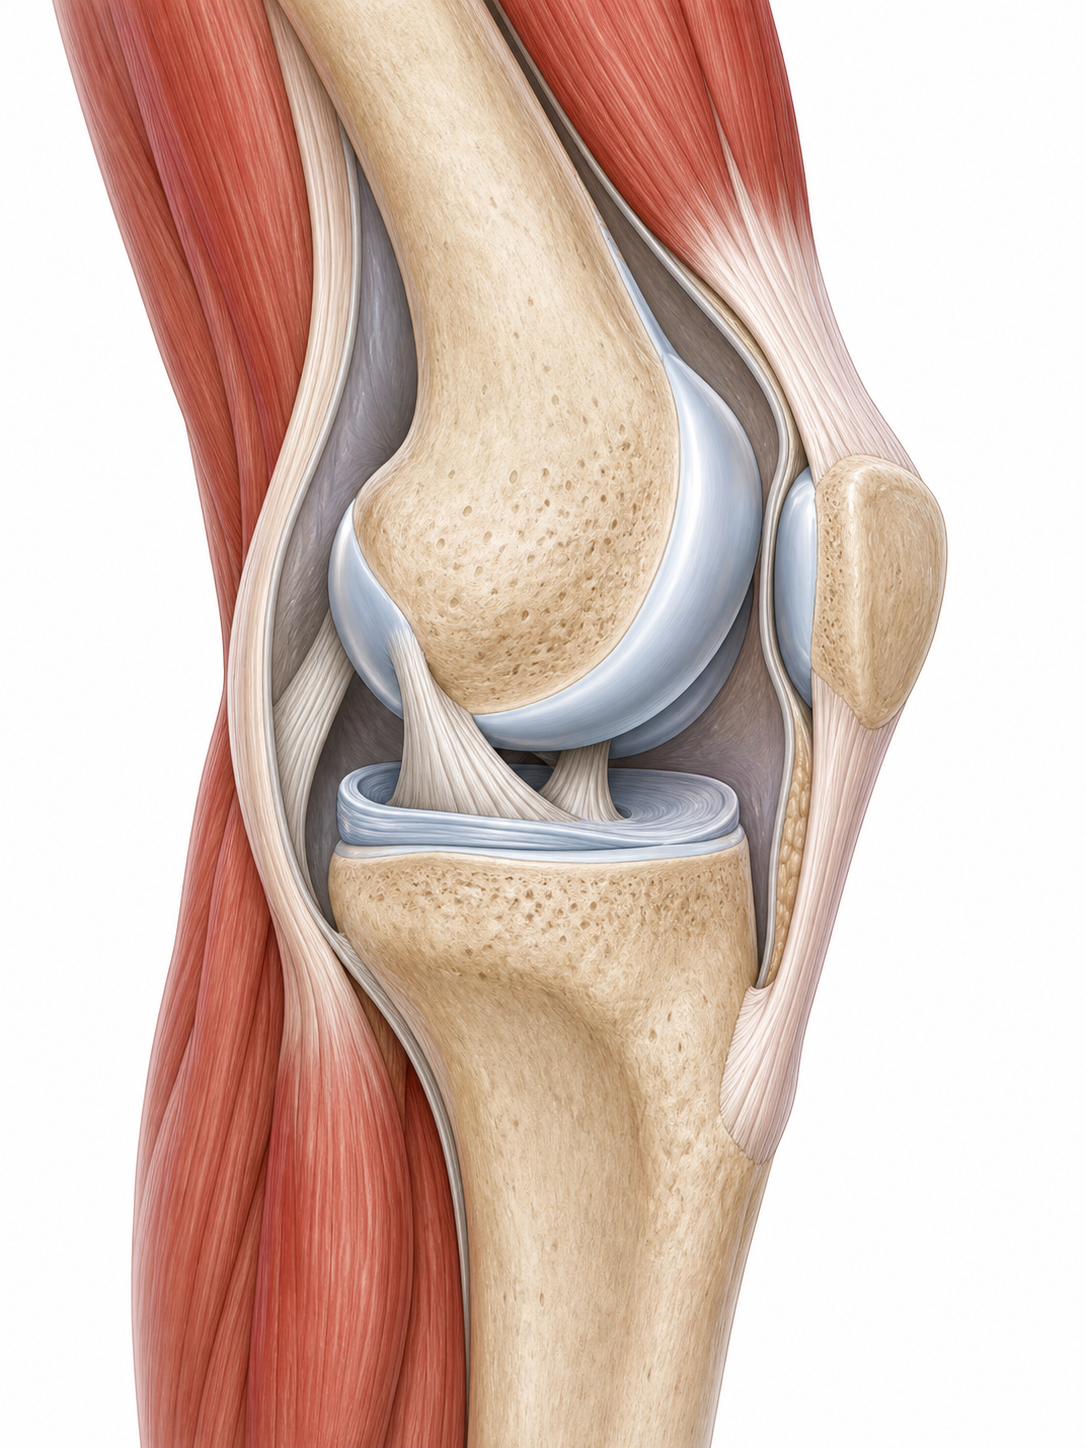
\includegraphics[width=0.4\linewidth]{images/book2/ai/fig-knee-cutaway.png}};
  \begin{scope}[x={(img.south east)}, y={(img.north west)},
      every node/.style={font=\small}]
    \draw[omDef, thick] (0.50,0.86) -- (1.05,0.90) node[right] {फ़ीमर};
    \draw[omDef, thick] (0.76,0.74) -- (1.05,0.74) node[right] {क्वाड्रिसेप्स कंडरा};
    \draw[omDef, thick] (0.82,0.58) -- (1.05,0.58) node[right] {पटेला};
    \draw[omDef, thick] (0.50,0.20) -- (1.05,0.14) node[right] {टिबिया};
    \draw[omDef, thick] (0.34,0.60) -- (-0.05,0.64) node[left] {उपास्थि};
    \draw[omDef, thick] (0.50,0.50) -- (-0.05,0.50) node[left] {स्नायु};
    \draw[omDef, thick] (0.40,0.44) -- (-0.05,0.36) node[left] {अर्धचंद्रक};
  \end{scope}
\end{tikzpicture}

{\small काट में घुटना: ऊपर फ़ीमर, नीचे टिबिया, और सामने जाँघ की पेशी की
\omterm{def:g10:muscles-and-joints:muscle}{कंडरा} में पटेला (घुटने की टोपी); हड्डियों के सिरों पर \omterm{def:g10:muscles-and-joints:joint}{उपास्थि}, उनके बीच
अर्धचंद्रक, और हड्डियों को जोड़े रखते \omterm{def:g10:muscles-and-joints:joint}{स्नायु}।}
\end{omfigure}

\begin{proposition}[हर हिस्सा किस काम का है]\label{prop:g10:muscles-and-joints:parts}
\omterm{def:g10:muscles-and-joints:joint}{उपास्थि} और श्लेष द्रव सतहों को बर्फ़ पर बर्फ़ से भी कम घर्षण के साथ
फिसलने देते हैं; अर्धचंद्रक उस भार को फैला देते हैं जो वरना कुछ ही वर्ग
मिलीमीटर पर सिमट जाता; \omterm{def:g10:muscles-and-joints:joint}{स्नायु} घुटने को मुड़ने और सीधा होने देते हैं पर
मरोड़ और बग़ल की ओर झुकाव का विरोध करते हैं; और संपुट द्रव को भीतर बनाए
रखता है। हर हिस्से की अपनी चूक है: \omterm{def:g10:muscles-and-joints:joint}{उपास्थि} घिसती है (संधिक्षय), मुड़े
हुए घुटने पर किसी मरोड़ में अर्धचंद्रक फटता है, और \omterm{def:g10:muscles-and-joints:joint}{संधि} को उसकी सीमा से
आगे धकेलने पर \omterm{def:g10:muscles-and-joints:joint}{स्नायु} में मोच आती है या वह टूट जाता है।
\end{proposition}
\admitted

\begin{example}[मोच, फटन, संधि-भ्रंश]\label{ex:g10:muscles-and-joints:injuries}
फुटपाथ के किनारे पर टख़ना मुड़ जाए: बाहर की ओर के \omterm{def:g10:muscles-and-joints:joint}{स्नायु} अपनी सीमा से आगे
खिंच जाते हैं --- यही \emph{मोच} है; और संपुट से ख़ून तथा द्रव जमा होने पर
\omterm{def:g10:muscles-and-joints:joint}{संधि} सूज जाती है। ठंडी हैमस्ट्रिंग को ज़ोर से खींचिए: उसके कुछ तंतु टूट
जाते हैं --- यानी पेशी की \emph{फटन}। फैली हुई बाँह पर गिरिए: ह्यूमरस का
सिर अपने खाँचे से बाहर आ सकता है --- यानी \emph{संधि-भ्रंश}, जिसमें
निकलते-निकलते \omterm{def:g10:muscles-and-joints:joint}{स्नायु} और संपुट खिंच या फट जाते हैं। इनमें से कोई हड्डी का
टूटना नहीं है; और सबको भरने में उससे अधिक समय लग सकता है।
\end{example}

\section{पेशियाँ खींचती हैं, जोड़ों में}

\begin{definition}[कंकाल पेशी और कंडरा]\label{def:g10:muscles-and-joints:muscle}
\emph{कंकाल पेशी}\index{कंकाल पेशी} एक अंग है जो हज़ारों लंबी \omterm{def:g10:cells-common-unit:cell}{कोशिकाओं},
यानी \emph{पेशी तंतुओं}, के गट्ठर से बना है; और हर तंतु किसी तंत्रिका के
उद्दीपन पर छोटा हो जाता है। दोनों सिरों पर पेशी सिकुड़कर
\emph{कंडरा}\index{कंडरा} बन जाती है, यानी बिना सिकुड़ने वाले ऊतक की एक
डोर, जो हड्डी से जुड़ी होती है। कोई पेशी केवल छोटी होकर \emph{खींच} सकती
है, और वह भी केवल अपनी ही लंबाई के साथ-साथ: वह किसी \omterm{def:g10:muscles-and-joints:joint}{संधि} को उसके आगे की
हड्डी पर खींचकर हिलाती है।
\end{definition}

\begin{proposition}[विरोधी जोड़े]\label{prop:g10:muscles-and-joints:antagonists}
चूँकि कोई पेशी धक्का नहीं दे सकती, इसलिए किसी \omterm{def:g10:muscles-and-joints:joint}{संधि} की हर हलचल के लिए एक
दूसरे के विरोध में काम करती दो पेशियाँ या दो समूह चाहिए: एक \emph{मोड़क},
जो \omterm{def:g10:muscles-and-joints:joint}{संधि} को मोड़ता है, और एक \emph{प्रसारक}, जो उसे सीधा करता है। जब एक
सिकुड़ती है तो दूसरी ढीली पड़कर खिंच जाती है; और कोई मुद्रा थामे रखने के
लिए दोनों साथ सिकुड़ती हैं। बाइसेप्स कोहनी को मोड़ता है और ट्राइसेप्स उसे
सीधा करता है; जाँघ के अगले हिस्से का क्वाड्रिसेप्स घुटने को सीधा करता है,
और उसके पीछे की हैमस्ट्रिंग उसे मोड़ती है।
\end{proposition}
\admitted

\begin{omfigure}
\begin{tikzpicture}[>=Stealth, font=\small, line cap=round]
  % upper arm (humerus) horizontal, forearm angled
  \draw[line width=7pt, gray!45] (0,0) -- (5,0);         % humerus
  \draw[line width=6pt, gray!45] (5,0) -- (8.6,2.0);     % forearm
  \fill[gray!60] (5,0) circle (0.28);
  \node[anchor=north] at (2.5,-0.25) {ह्यूमरस};
  \node[anchor=north west] at (7.2,1.1) {अग्रबाहु};
  \node[anchor=west] at (5.5,-0.5) {कोहनी};
  % biceps: from shoulder region above humerus to forearm just past elbow
  \draw[line width=9pt, omThm!60] (0.6,0.6) .. controls (3,1.4) .. (5.35,0.9);
  \draw[thick, omThm!80!black] (5.35,0.9) -- (5.65,0.45);   % tendon
  \node[omThm!80!black, anchor=south] at (3,1.3) {बाइसेप्स (मोड़क): सिकुड़ता है};
  % triceps: below humerus to the back of the forearm
  \draw[line width=7pt, omDef!50] (0.6,-0.9) .. controls (3,-1.6) .. (4.9,-1.0);
  \draw[thick, omDef!80!black] (4.9,-1.0) -- (5.25,-0.4);
  \node[omDef!80!black, anchor=north] at (3,-1.65) {ट्राइसेप्स (प्रसारक): ढीला पड़कर खिंचता है};
  \draw[->, thick] (8.6,2.0) to[bend right=20] (8.0,3.0);
  \node[anchor=south] at (8.3,3.05) {मोड़};
  \draw[->, thick, omThm!80!black] (5.65,0.45) -- (5.2,0.75);
\end{tikzpicture}

{\small कोहनी पर एक विरोधी जोड़ा। बाइसेप्स, जो \omterm{def:g10:muscles-and-joints:joint}{संधि} से ज़रा आगे अग्रबाहु
से जुड़ा है, छोटा होकर कोहनी मोड़ देता है; और ट्राइसेप्स, जो \omterm{def:g10:muscles-and-joints:joint}{संधि} के पीछे
जुड़ा है, ढीला पड़कर खिंच जाता है। बाँह सीधी करने के लिए दोनों की
भूमिकाएँ उलट दीजिए।}
\end{omfigure}

\begin{proposition}[उत्तोलक और बल]\label{prop:g10:muscles-and-joints:lever}
किसी \omterm{def:g10:muscles-and-joints:joint}{संधि} पर घूमती हड्डी एक उत्तोलक है। पेशी की \omterm{def:g10:muscles-and-joints:muscle}{कंडरा} धुरी से थोड़ी दूरी
$d$ पर जुड़ती है, जबकि भार उससे बड़ी दूरी $D$ पर लगता है; और संतुलन के
लिए पेशी को इतने बल से खींचना पड़ता है
\[
F_{\text{पेशी}} = F_{\text{भार}} \times \frac{D}{d},
\]
जो भार से कई गुना है। यह बंदोबस्त बल के बदले रफ़्तार और परास ख़रीदता है:
पेशी का ज़रा-सा छोटा होना हाथ या पैर की एक बड़ी, तेज़ हलचल बना देता है,
और उसका दाम \omterm{def:g10:muscles-and-joints:muscle}{कंडरा} तथा \omterm{def:g10:muscles-and-joints:joint}{संधि} में लगने वाले बड़े बल हैं।
\end{proposition}
\admitted

\begin{example}[थैला थामना]\label{ex:g10:muscles-and-joints:bag}
\qty{5}{kg} का एक थैला (भार \qty{49}{N}) हाथ से लटका है, कोहनी से
\qty{35}{cm} दूर; और बाइसेप्स की \omterm{def:g10:muscles-and-joints:muscle}{कंडरा} कोहनी से \qty{5}{cm} पर जुड़ी है।
बाइसेप्स $49 \times 35/5 = \qty{343}{N}$ से खींचता है --- यानी भार का
सात गुना, जो \qty{35}{kg} के भार जितना है --- और कोहनी की \omterm{def:g10:muscles-and-joints:joint}{संधि} लगभग
\qty{300}{N} से आपस में दबती है। पेशियाँ, \omterm{def:g10:muscles-and-joints:muscle}{कंडराएँ} और \omterm{def:g10:muscles-and-joints:joint}{उपास्थि} इन्हीं बलों
के लिए बनी हैं; उन्हें नुक़सान ग़लत दिशा का कोई अचानक बल पहुँचाता है, या
इतनी बार दोहराया गया भार कि ऊतक उसकी मरम्मत ही न कर सके।
\end{example}

\begin{omfigure}
\begin{tikzpicture}[>=Stealth, font=\small]
  \draw[line width=6pt, gray!45] (0,0) -- (7,0);
  \fill[gray!70] (0,0) circle (0.25);
  \node[anchor=north] at (0,-0.35) {कोहनी (धुरी)};
  \draw[->, very thick, omThm] (1,0.15) -- (1,2.2) node[above] {$F_{\text{पेशी}}$};
  \draw[->, very thick, omDef] (7,-0.15) -- (7,-1.6) node[below] {$F_{\text{भार}} = \qty{49}{N}$};
  \draw[<->] (0,0.9) -- (1,0.9) node[midway, above, xshift=-4mm] {$d = \qty{5}{cm}$};
  \draw[<->] (0,-1.25) -- (7,-1.25) node[midway, below] {$D = \qty{35}{cm}$};
\end{tikzpicture}

{\small उत्तोलक के रूप में अग्रबाहु: बाइसेप्स धुरी के पास खींचता है, और
भार उससे दूर लटकता है। $F_{\text{पेशी}} \times d =
F_{\text{भार}} \times D$, इसलिए पेशी का बल भार का $D/d = 7$ गुना है।}
\end{omfigure}

\section{पेशी के भीतर}

\begin{proposition}[पेशी तंतु की बनावट]\label{prop:g10:muscles-and-joints:fibre}
\omterm{def:g10:muscles-and-joints:muscle}{पेशी तंतु} अकेली एक विशाल \omterm{def:g10:cells-common-unit:cell}{कोशिका} है, \num{10}--\qty{100}{\micro m}
चौड़ी और कई सेंटीमीटर तक लंबी, जिसमें बहुत-से \omterm{def:g10:cells-common-unit:organelle}{केंद्रक} होते हैं। वह समांतर
\emph{पेशीतंतुकों} से ठसाठस भरी है, और हर पेशीतंतुक दोहराई जाती इकाइयों
की एक शृंखला है जिसमें दो तरह के \omterm{def:g10:chemistry-of-life:families}{प्रोटीन} तंतुक, मोटे और पतले, एक-दूसरे
में घुसे रहते हैं। संकुचन इन्हीं पतले तंतुकों का मोटे तंतुकों के बीच
सरकना है, जिसे ATP चलाता है: हर इकाई एक अंश भर छोटी होती है, पेशीतंतुक
उनके योग भर, और तंतु उसके साथ। पेशीतंतुकों के बीच की \omterm{def:g10:cells-common-unit:organelle}{सूत्रकणिकाएँ} ATP
देती हैं; और हर तंतु पर बैठा एक तंत्रिका सिरा आदेश देता है।
\end{proposition}
\admitted

\begin{omfigure}
\begin{tikzpicture}[font=\small, >=Stealth]
  \tikzset{lvl/.style={draw, rounded corners, thick, align=center, minimum height=1.1cm}}
  \node[lvl, fill=omThm!12, text width=2.1cm] (m) at (0,0) {पेशी\\ (अंग)};
  \node[lvl, fill=omThm!12, text width=2.1cm] (b) at (3.0,0) {तंतुओं का\\ गट्ठर};
  \node[lvl, fill=omProp!15, text width=2.1cm] (f) at (6.0,0) {पेशी तंतु\\ (एक कोशिका)};
  \node[lvl, fill=omDef!12, text width=2.1cm] (my) at (9.0,0) {पेशीतंतुक};
  \node[lvl, fill=omMeth!15, text width=2.1cm] (fi) at (12.0,0) {मोटे और पतले\\ तंतुक};
  \foreach \a/\b in {m/b, b/f, f/my, my/fi} \draw[->] (\a) -- (\b);
  \node[anchor=north, font=\scriptsize] at (m.south) {सेंटीमीटर};
  \node[anchor=north, font=\scriptsize] at (b.south) {मिलीमीटर};
  \node[anchor=north, font=\scriptsize] at (f.south) {\qty{50}{\micro m} चौड़ा};
  \node[anchor=north, font=\scriptsize] at (my.south) {\qty{1}{\micro m} चौड़ा};
  \node[anchor=north, font=\scriptsize] at (fi.south) {\qty{10}{nm}};
\end{tikzpicture}

{\small पूरी पेशी से लेकर उन अणुओं तक जो उसे छोटा करते हैं: संगठन के पाँच
स्तर, और हर स्तर अगले का गट्ठर। तंतुकों का एक-दूसरे के पास से सरकना, हर
इकाई पर दोहराया हुआ, ही संकुचन है।}
\end{omfigure}

\begin{definition}[तंतुओं के प्रकार]\label{def:g10:muscles-and-joints:types}
\omterm{def:g10:muscles-and-joints:muscle}{पेशी तंतु} मुख्यतः दो प्रकार के होते हैं। \emph{धीमे तंतु} धीरे और कमज़ोर
सिकुड़ते हैं पर बिना थके: \omterm{def:g10:cells-common-unit:organelle}{सूत्रकणिकाओं} और केशिकाओं से भरपूर, ऑक्सीजन
सँभालने वाले किसी \omterm{def:g10:chemistry-of-life:families}{प्रोटीन} से लाल, वे श्वसन पर चलते हैं और मुद्रा सँभालने
वाली पेशियों तथा सहनशक्ति के खिलाड़ियों में छाए रहते हैं। \emph{तेज़
तंतु} जल्दी और ज़ोर से सिकुड़ते हैं पर मिनट भर में थक जाते हैं:
\omterm{def:g10:cells-common-unit:organelle}{सूत्रकणिकाओं} में ग़रीब, रंग में फीके, वे फ़ॉस्फ़ेट भंडार और \omterm{def:g10:cell-metabolism:fermentation}{किण्वन} के
भरोसे रहते हैं और फ़र्राटा धावकों में छाए रहते हैं। किसी दी हुई पेशी में
इनका अनुपात बड़े हिस्से में वंशागत होता है; प्रशिक्षण तंतुओं की संख्या से
कहीं अधिक उनका आकार और साज़-सामान बदलता है।
\end{definition}

\begin{example}[पेशी की बायोप्सी पढ़ना]\label{ex:g10:muscles-and-joints:biopsy}
जाँघ की पेशी की पतली फाँक पर \omterm{def:g10:cells-common-unit:organelle}{सूत्रकणिका} के एंजाइमों का रंजक एक मोज़ेक
दिखाता है: गहरे तंतु (धीमे) और फीके तंतु (तेज़)। किसी मैराथन धावक का
नमूना 80\% गहरा होता है; किसी फ़र्राटा धावक का 30\%; और बिना प्रशिक्षण
वाले व्यक्ति का लगभग आधा-आधा। साल भर के फ़र्राटा प्रशिक्षण के बाद उसी
धावक पर वही रंजक फीके तंतुओं को बड़ा हुआ दिखाता है, संख्या में अधिक नहीं।
\end{example}

\section{थकान, नुक़सान, मरम्मत}

\begin{proposition}[पेशी की सीमाएँ]\label{prop:g10:muscles-and-joints:limits}
पेशी तीन अलग-अलग ढंग से चूकती है। \emph{थकान}: जब ATP की आपूर्ति साथ नहीं
दे पाती तो बल गिर जाता है --- तेज़ तंतुओं में मिनट भर के भीतर, धीमों में
घंटों में --- और विश्राम से वह लौट आता है। \emph{ऐंठन}: कोई अचानक, टिका
हुआ, अनैच्छिक संकुचन, जो अक्सर निर्जलीकरण या लवण की हानि से होता है।
\emph{चोट}: तंतु ऐसे बल से टूटते हैं जो उनकी ताक़त से बड़ा हो, और आमतौर
पर तब जब पेशी ठंडी, थकी हुई, या सिकुड़ते-सिकुड़ते खिंची हुई हो। तंतु पेशी
की आरक्षित \omterm{def:g10:cells-common-unit:cell}{कोशिकाओं} से हफ़्तों में मरम्मत हो जाते हैं; पर \omterm{def:g10:muscles-and-joints:muscle}{कंडरा} या \omterm{def:g10:muscles-and-joints:joint}{स्नायु},
जिन तक ख़ून कम पहुँचता है, महीनों में।
\end{proposition}
\admitted

\begin{method}[किसी पेशी-कंकाल चोट का विश्लेषण]\label{met:g10:muscles-and-joints:analyse}
\begin{enumerate}
  \item जिस हलचल ने उसे किया उसे और उसकी दिशा को पहचानिए: क्या \omterm{def:g10:muscles-and-joints:joint}{संधि} अपनी
        परास के भीतर हिली (यानी पेशी की समस्या) या उससे आगे (यानी \omterm{def:g10:muscles-and-joints:joint}{स्नायु}
        या संपुट की समस्या)?
  \item ऊतक पहचानिए: \omterm{def:g10:muscles-and-joints:muscle}{पेशी तंतु} टूटते हैं (पेशी के पेट में दर्द,
        कमज़ोरी); \omterm{def:g10:muscles-and-joints:joint}{स्नायु} में मोच आती है (\omterm{def:g10:muscles-and-joints:joint}{संधि} पर दर्द और सूजन,
        अस्थिरता); \omterm{def:g10:muscles-and-joints:muscle}{कंडराएँ} दोहराए गए भार से सूज जाती हैं; और \omterm{def:g10:muscles-and-joints:joint}{उपास्थि}
        सालों तक चुपचाप घिसती रहती है।
  \item बल आँकिए: उत्तोलक का नियम लगाइए; और याद रखिए कि ज़मीन पर उतरना
        या रुकना शरीर के भार को कई गुना कर देता है।
  \item ऊतक तक ख़ून की पहुँच से उबरने का अनुमान लगाइए: पेशी हफ़्तों में,
        \omterm{def:g10:muscles-and-joints:joint}{स्नायु} और \omterm{def:g10:muscles-and-joints:muscle}{कंडरा} महीनों में, और \omterm{def:g10:muscles-and-joints:joint}{उपास्थि} शायद ही कभी।
\end{enumerate}
\end{method}

\begin{remark}[गरमाना काम क्यों करता है]\label{rem:g10:muscles-and-joints:warmup}
दस मिनट की हल्की हलचल पेशियों का ताप एक-दो अंश बढ़ा देती है, जिससे उनके
\omterm{def:g10:chemistry-of-life:families}{प्रोटीन} अधिक खिंचाऊ और उनके \omterm{def:g10:cell-metabolism:metabolism}{एंजाइम} तेज़ हो जाते हैं; वह उन केशिकाओं को
खोल देती है जो \cref{ch:g10:heart-lungs-effort} वाली ऑक्सीजन पहुँचाएँगी;
और वह \omterm{def:g10:muscles-and-joints:joint}{उपास्थि} पर श्लेष द्रव की परत मोटी कर देती है। ठंडी पेशी से अधिकतम
संकुचन माँगना फटन का सबसे आम कारण है; और जिस \omterm{def:g10:muscles-and-joints:joint}{संधि} पर उसका द्रव फैलने से
पहले भार पड़े, वह जल्दी घिसती है।
\end{remark}

\section{अभ्यास}

\begin{exercise}[$\star$]\label{exo:g10:muscles-and-joints:1}
किसी चलायमान \omterm{def:g10:muscles-and-joints:joint}{संधि} के हिस्सों के नाम लिखिए और हर एक की भूमिका बताइए।
\end{exercise}

\begin{exercise}[$\star$]\label{exo:g10:muscles-and-joints:2}
\omterm{def:g10:muscles-and-joints:muscle}{कंडरा} और \omterm{def:g10:muscles-and-joints:joint}{स्नायु} में क्या अंतर है?
\end{exercise}

\begin{exercise}[$\star$]\label{exo:g10:muscles-and-joints:3}
हर \omterm{def:g10:muscles-and-joints:joint}{संधि} को हिलने के लिए कम से कम दो पेशियाँ क्यों चाहिए?
\end{exercise}

\begin{exercise}[$\star$]\label{exo:g10:muscles-and-joints:4}
शामिल ऊतक के आधार पर मोच, पेशी की फटन और संधि-भ्रंश में अंतर बताइए।
\end{exercise}

\begin{exercise}[$\star$]\label{exo:g10:muscles-and-joints:5}
धीमे और तेज़ \omterm{def:g10:muscles-and-joints:muscle}{पेशी तंतुओं} के बीच दो फ़र्क़ बताइए।
\end{exercise}

\begin{exercise}[$\star\star$]\label{exo:g10:muscles-and-joints:6}
\qty{2}{kg} का एक डंबल हाथ में थामा गया है, कोहनी से \qty{32}{cm} दूर;
और बाइसेप्स कोहनी से \qty{4}{cm} पर जुड़ता है। बाइसेप्स में बल निकालिए
($g = \qty{9.8}{N/kg}$)।
\end{exercise}

\begin{exercise}[$\star\star$]\label{exo:g10:muscles-and-joints:7}
समझाइए कि किसी अनपेक्षित धक्के के सामने बाँह को स्थिर थामे रखने के लिए
बाइसेप्स और ट्राइसेप्स, दोनों को क्यों सिकुड़ना पड़ता है।
\end{exercise}

\begin{exercise}[$\star\star$]\label{exo:g10:muscles-and-joints:8}
\qty{3}{cm} लंबा कोई \omterm{def:g10:muscles-and-joints:muscle}{पेशी तंतु} सिकुड़ने पर 20\% छोटा हो जाता है। यदि उस
तंतु की \omterm{def:g10:muscles-and-joints:muscle}{कंडरा} कोहनी से \qty{5}{cm} पर जुड़ी हो और हाथ कोहनी से
\qty{35}{cm} दूर हो, तो हाथ कितना हिलेगा?
\end{exercise}

\begin{exercise}[$\star\star$]\label{exo:g10:muscles-and-joints:9}
कंधा, जो शरीर की सबसे चलायमान \omterm{def:g10:muscles-and-joints:joint}{संधि} है, सबसे अधिक बार अपने स्थान से भी
क्यों हट जाता है?
\end{exercise}

\begin{exercise}[$\star\star$]\label{exo:g10:muscles-and-joints:10}
गरम मौसम की किसी दौड़ के अंत में धावक की पिंडली की पेशी में ऐंठन आ जाती
है। अध्याय से दो कारण और एक उपाय सुझाइए।
\end{exercise}

\begin{exercise}[$\star\star$]\label{exo:g10:muscles-and-joints:11}
\cref{ex:g10:muscles-and-joints:biopsy} की मदद से समझाइए कि मैराथन का
प्रशिक्षण लेता कोई फ़र्राटा धावक उसी उम्र के बिना प्रशिक्षण वाले
व्यक्ति से कम क्यों सुधरता है।
\end{exercise}

\begin{exercise}[$\star\star\star$]\label{exo:g10:muscles-and-joints:12}
किसी छलाँग से उतरते समय घुटना मुड़ता है और क्वाड्रिसेप्स की \omterm{def:g10:muscles-and-joints:muscle}{कंडरा} शरीर के
भार का लगभग चार गुना ढोती है। \qty{70}{kg} के खिलाड़ी के लिए वह बल
निकालिए। \omterm{def:g10:muscles-and-joints:muscle}{कंडरा} का अनुप्रस्थ काट लगभग \qty{1}{cm^2} है और वह क़रीब
\qty{100}{N/mm^2} पर टूटती है; वह टूटने से कितनी दूर है?
\end{exercise}

\begin{exercise}[$\star\star\star$]\label{exo:g10:muscles-and-joints:13}
फटा हुआ \omterm{def:g10:muscles-and-joints:joint}{स्नायु} महीनों में भरता है, फटी हुई पेशी हफ़्तों में, और घिसी हुई
\omterm{def:g10:muscles-and-joints:joint}{उपास्थि} शायद ही कभी। इन तीनों को ऊतकों तक ख़ून की पहुँच और मरम्मत के लिए
उपलब्ध \omterm{def:g10:cells-common-unit:cell}{कोशिकाओं} से जोड़िए।
\end{exercise}

\begin{exercise}[$\star\star\star$]\label{exo:g10:muscles-and-joints:14}
शरीर-सौष्ठव पेशियों को बड़ा करता है; और खिंचाव \omterm{def:g10:muscles-and-joints:joint}{संधि} की परास बढ़ाता है।
इनमें से हर एक किस ऊतक को बदलता है, और दोनों में से कोई तंतुओं की संख्या
क्यों नहीं बदलता?
\end{exercise}

\begin{exercise}[$\star\star\star$]\label{exo:g10:muscles-and-joints:15}
किसी बुज़ुर्ग के घुटने की \omterm{def:g10:muscles-and-joints:joint}{उपास्थि} घिसकर अपनी आधी मोटाई रह गई है। अध्याय
से समझाइए कि सीढ़ियों पर \omterm{def:g10:muscles-and-joints:joint}{संधि} क्यों दुखती है, अर्धचंद्रक पहले से अधिक
क्यों मायने रखते हैं, और घुटने के इर्द-गिर्द की पेशियाँ इलाज का हिस्सा
क्यों हैं।
\end{exercise}

\section{समस्या: किसी घुटने के भीतर के बल}

\begin{problem}[{सप्ताहांत समस्या --- किसी फ़ुटबॉल खिलाड़ी का घुटना खोलकर
देखा गया: टाँग का उत्तोलक, जाँघ की पेशी की खींच, वह स्नायु जो फटा, और वे
अंक जो कोई कंडरा हर क़दम पर ढोती है}]
\label{pb:g10:muscles-and-joints:1}
\qty{70}{kg} के करीम ने जमे हुए पैर पर तेज़ी से मुड़ते हुए अपना घुटना
चोटिल कर लिया। $g = \qty{9.8}{N/kg}$ लीजिए। क्वाड्रिसेप्स की \omterm{def:g10:muscles-and-joints:muscle}{कंडरा}
टिबिया से घुटने की धुरी से \qty{5}{cm} पर जुड़ती है; और घुटना अच्छी तरह
मुड़ा हो, जैसा उतरते समय होता है, तो ज़मीन का पैर पर धक्का धुरी से लगभग
\qty{20}{cm} पर लगता है।

\medskip
\noindent\textbf{भाग I --- खड़े होना और क़दम रखना।}
\begin{enumerate}
  \item करीम का भार निकालिए।
  \item ज़रा मुड़े घुटने के साथ एक टाँग पर खड़े होने पर ज़मीन पैर को
        उसके पूरे भार से ऊपर धकेलती है, और वह धुरी से \qty{10}{cm} पर
        लगता है। क्वाड्रिसेप्स की \omterm{def:g10:muscles-and-joints:muscle}{कंडरा} में बल निकालिए।
  \item सीढ़ी चढ़ते समय घुटना और अधिक मुड़ता है और ज़मीन का बल धुरी से
        \qty{20}{cm} पर लगता है। \omterm{def:g10:muscles-and-joints:muscle}{कंडरा} का बल फिर से निकालिए।
  \item दोनों नतीजों को शरीर के भार के गुणकों में लिखिए, और समझाइए कि
        सीढ़ियाँ जाँघों को क्यों थका देती हैं।
  \item क्वाड्रिसेप्स का विरोधी कौन-सा पेशी समूह है, और क़दम के दौरान वह
        क्या कर रहा होता है?
\end{enumerate}

\medskip
\noindent\textbf{भाग II --- उतरना।}
\begin{enumerate}[resume]
  \item हेडर के बाद उतरते समय ज़मीन करीम के भार से तिगुने बल से धक्का
        देती है, धुरी से \qty{20}{cm} पर। \omterm{def:g10:muscles-and-joints:muscle}{कंडरा} का बल निकालिए।
  \item \omterm{def:g10:muscles-and-joints:muscle}{कंडरा} का अनुप्रस्थ काट \qty{1.2}{cm^2} है। उसमें प्रतिबल न्यूटन
        प्रति वर्ग मिलीमीटर में निकालिए, और लगभग \qty{100}{N/mm^2} के
        टूटने वाले प्रतिबल से तुलना कीजिए।
  \item \omterm{def:g10:muscles-and-joints:joint}{संधि} की सतहें मोटे तौर पर \omterm{def:g10:muscles-and-joints:muscle}{कंडरा} के बल और ज़मीन के बल के योग से
        आपस में दबती हैं। वह भार निकालिए, फिर \omterm{def:g10:muscles-and-joints:joint}{उपास्थि} पर दाब भी, यदि
        संपर्क का क्षेत्रफल अर्धचंद्रकों के साथ \qty{6}{cm^2} और उनके
        बिना \qty{1}{cm^2} हो।
  \item इससे निकालिए कि जिस घुटने का अर्धचंद्रक जा चुका हो उसकी \omterm{def:g10:muscles-and-joints:joint}{उपास्थि}
        तेज़ी से क्यों घिसती है।
  \item समझाइए कि उतरते समय श्लेष द्रव का क्या योगदान होता है।
\end{enumerate}

\medskip
\noindent\textbf{भाग III --- चोट।}
\begin{enumerate}[resume]
  \item करीम का पैर जमा था और उसका शरीर मुड़ा: घुटने पर किस दिशा की
        हलचल थोपी गई, और उसका विरोध करने के लिए कौन-सा ऊतक बना है?
  \item क्वाड्रिसेप्स, जो कई किलोन्यूटन से खींच सकता है, \omterm{def:g10:muscles-and-joints:joint}{स्नायु} को क्यों
        नहीं बचा पाया?
  \item घुटना घंटे भर में सूज गया। उसे किसने भरा, और \omterm{def:g10:muscles-and-joints:joint}{संधि} का कौन-सा
        हिस्सा टूटा था?
  \item स्कैन दिखाता है कि \omterm{def:g10:muscles-and-joints:joint}{स्नायु} टूट गया है और एक अर्धचंद्रक फट गया है।
        \cref{met:g10:muscles-and-joints:analyse} की मदद से हर एक के
        उबरने का समय बताइए और उसे उन तक ख़ून की पहुँच से समझाइए।
  \item करीम पूछता है कि सर्जन ऑपरेशन से पहले उसकी हैमस्ट्रिंग मज़बूत
        क्यों करना चाहता है। \cref{prop:g10:muscles-and-joints:antagonists}
        से जवाब दीजिए।
\end{enumerate}

\medskip
\noindent\textbf{भाग IV --- हर क़दम गिना जाता है।}
\begin{enumerate}[resume]
  \item करीम दिन भर में लगभग 8000 क़दम चलता है; आधे चोटिल टाँग पर।
        प्रश्न 2 वाले बल की मदद से बताइए कि \omterm{def:g10:muscles-and-joints:muscle}{कंडरा} दिन में कितनी बार कम
        से कम उतना भार ढोती है।
  \item साल भर में कुल कितनी बार भार पड़ता है? समझाइए कि अति-प्रयोग से
        सूजी हुई \omterm{def:g10:muscles-and-joints:muscle}{कंडरा} (कंडराशोथ) को ताक़त के बजाय आराम क्यों चाहिए।
  \item किसी मैच में वह क़रीब 40 बार छलाँगों से उतरता है। उतरने में
        (प्रश्न 6) ढोए गए कुल भार की तुलना दिन भर के क़दमों में ढोए गए
        भार से कीजिए।
  \item दौड़ना चलने के मुक़ाबले ज़मीन के बल को दोगुना कर देता है।
        डॉक्टर भरते हुए घुटने के लिए दौड़ने के बजाय साइकिल चलाने और
        तैरने की सलाह क्यों देते हैं?
  \item परिणाम लिखिए: सीढ़ी पर और उतरते समय क्वाड्रिसेप्स की \omterm{def:g10:muscles-and-joints:muscle}{कंडरा} शरीर
        के भार का कितना गुना ढोती है, और घुटने का वह एक ऊतक कौन-सा है
        जिसकी ताक़त इन अंकों ने कभी नहीं परखी --- उस मोड़ तक।
\end{enumerate}
\end{problem}
